\chapter{Technical frame}
\label{chap:ch3}

\section{Backend}

\subsection{.NET and ASP.NET Core}

\par .NET (pronounced as "dot net") is a free, cross-platform, open-source developer platform for building many kinds of applications including web, desktop, mobile, cloud, IoT. It can run programs written in multiple languages, with C\# being the most popular. It relies on a high-performance runtime that is used in production by many high-scale apps. \cite{microsoftIntroDotNet} It was released in 2016 and its the successor of .NET Framework which dates way back to 2002.

\par ASP.NET Core is a free, cross-platform, open-source framework for building web apps and services with .NET and C\#. It is part of the app stack provided by .NET. Key features are: dependency injection, middleware pipeline, MVC, security.

\subsection{Entity Framework Core}

\par Entity Framework Core (EF Core) is an open source and cross-platform Object-Relational Mapping (ORM) framework for .NET applications. It is the successor to the original Entity Framework (EF) and has been redesigned to be lightweight and extensible. EF Core allows developers to work with a database using .NET objects, eliminating the need to write most of the data-access code manually. Key concepts:

\par \textbf{DbContext} is the primary class reponsible for interacting with the database. It manages the entity objects during runtime, tracks changes, handles the database interaction and allows customization of the ORM behavior.

\par \textbf{DbSet\textless{T}\textgreater{}} class represents a collection of entities of a specific type (`T`). Each DbSet in a DbContext corresponds to a table in the database and entity instance corresponds to a row in that table.

\begin{sloppypar} % in ordet to fix overflow
\par \textbf{Entities} are classes that map to tables in a relational database. Each property in an entity class corresponds to a column in the table (with certain exceptions, since EF allows defining a more complex behavior, as stated in  \url{https://learn.microsoft.com/en-us/ef/core/modeling/backing-field}) and each instance of the class corresponds to a row.
\end{sloppypar}


\par \textbf{LINQ (Language Integrated Query)} is used to query the database in a types-safe and object-oriented manner. It allows developers to write queries against the DbContext using standard C\# syntax:

\begin{figure}[!ht]
    \centering
    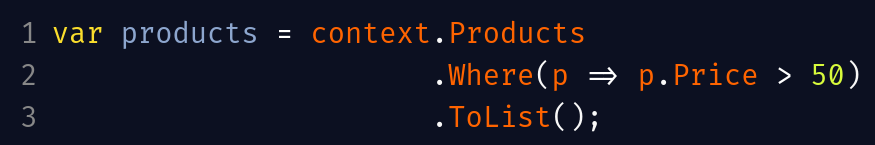
\includegraphics[width=1\linewidth]{linq-example.png}
\end{figure}

\par \textbf{Migrations} is a feature that helps managing database schema changes over the database's life-cycle. They allow you to incrementally apply changes to the schema, such as adding new tables, modifying columns, creating relationships between tables, etc, while preserving exitsting data.

\par \textbf{Change tracking}: EF Core automatically keeps track of changes made to entities during the lifetime of a DbContext instances. When \textit{SaveChanges()} is called, EF Core determines what changes have been made and generates the appropriate SQL commands to update the database.

\par \textbf{Relationships}: EF Core allows you to define relationships between entities, such as one-to-one, one-to-many, and many-to-many relationships. These relationships are represented using navigation properties and are enforced through foreign keys in the database.

\subsection{Frontend}

\subsubsection{React}

\par React is an open-source front-end JavaScript library released in 2013 by Meta (formerly Facebook). Back in 2011, the developers at Facebook started to face some issues with code maintenance. Which was caused by the increase in app features combined with cascading updates. The solution they arrived at is React. \cite{reactHistory} React does things by breaking down the UI into reusable components. This component-based architecture allows to build complex user interfaces by composing small, isolated pieces of code that manage their own state and logic. Key concepts:

\par \textbf{JSX} (\textbf{JavaScript XML}, formally \textbf{JavaScript Syntax eXtension}) is an XML-like extension to the JavaScript language syntax. \cite{jsx} It just a syntatic sugar that is transpiled into nested JavaScript function calls structurally similar to the original JSX. JSX lets you write HTML-like markup inside a JavaScript file. Inside React, it is used to define components.

\par \textbf{Components} are the UI building blocks in React. They are self-contained pieces of UI that can be reused throughout the application and are defined using JSX. They can be either functional (as the return of a function) or class-based (created by extending React.Component). Throughout the app, only functional components are used. Example of a functional component:

\begin{figure}[!ht]
    \centering
    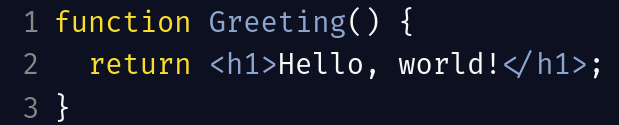
\includegraphics[width=1\linewidth]{react-component-example.png}
\end{figure}

\par \textbf{Props} (short for properties) are read-only data passed from a parent component to a child component. Props allow components to be dynamic and reusable by passing different data into them.

\par \textbf{Hooks} are function provided by the React API that provide features like "remembering" information like user input (useState), receiving information from a distant parent without passing it as props (useContext), holding information that isn't used for rendering (useRef), connecting to and synchronizing with external systems (useEffect). \cite{reactHooks}

\par \textbf{State} represents the internal writable data insides a component. State is declared using the \textbf{useState} hook which returns 2 the value of the state and a function to set that value. The value can be used directly in the JSX or to compute some other state. The setter should only be called inside other hooks or event handlers and not during rendering (i.e. directly inside functional components, which should be pure functions).

\par \textbf{Virtual DOM} In case of big pages, re-rendering can become an expensive operation. That's why react uses a virtual DOM, which is a copy of the real DOM. When the state of a component changes, a snapshot of its current virtual DOM is saved, then the virtual DOM is modified and compared with the snapshot and only then, the real DOM is changed based on the difference between the initial and the modified virtual DOM.

\subsubsection{TypeScript}

\par TypeScript is a strongly typed, compiled programming language that builds on JavaScript, one of the most widely used languages for web development. Developed and maintained by Microsoft, TypeScript introduces static typing to JavaScript, along with other features aimed at improving developer productivity and code maintainability. It has rapidly gained popularity in the web development community and is commonly used in conjunction with frameworks such as Angular, React, and Vue.js.

\par TypeScript is a superset of JavaScript, meaning any valid JavaScript code is also valid TypeScript code. TypeScript’s main feature is its optional static typing, which allows developers to define the types of variables, function parameters, and function return values. This helps catch errors at compile time rather than at runtime, leading to more robust and maintainable code.

\par TypeScript is transpiled into plain JavaScript, which can run in any environment that supports JavaScript, including web browsers, Node.js, and various JavaScript engines. The TypeScript compiler checks the code for type errors and compiles it into JavaScript that is compatible with the target environment.

\par TypeScript has type inference, which means the compiler can deduce the types of variables based on the values they are assigned. It also introduces interfaces, type aliases, access modifiers, generics and ES6 modules.

\par Using TypeScript comes with the advantage of strong typing, but the disadvantages are: the learning curve, the compilation step - converting the TypeScript code to JavaScript, which adds an extra layer of complexity to the development workflow and the dependency management.

\subsubsection{Redux}

\par Redux is an open-source JavaScript library for managing and centralizing application state. In React, centralized state management can be achieved to some degree using the \textit{useContext} feature. But, for medium to large-sized codebases with large amounts of application state and frequent and complex update logic, that might become too complex to maintain. Redux uses a single source of truth which contains read-only state that can only be modified through pure functions called reducers. The core components of Redux are the following:

\begin{itemize}
    \item Store - is the central object that holds the application’s state. It is created using the \textit{createStore} function provided by Redux. The store provides methods to access the state, dispatch actions, and subscribe to changes.
    \item State - is a single JavaScript object that represents the entire application’s data. It can only be updated by dispatching actions and processing those actions in reducers.
    \item Actions - are plain JavaScript objects that describe what happened in the application. Each action has a type property (a string constant) and can optionally have a payload property that carries additional data. Actions are dispatched to the store to trigger state changes.
    \item Reducers - are pure functions that take the current state and an action as inputs and return a new state. Reducers specify how the state should change in response to an action. Since reducers are pure functions, they do not modify the original state but return a new state object.
\end{itemize}

\par When a value in the state affects what is displayed to the user (example: the number of items in a shopping cart), that means that state defines the UI. When a user interacts with the page, by clicking a button or inputting text, an action is triggered (example: adding an item to the shopping cart). This action is dispatched to a reducer (example: the reducer receives an action of type addItemToCart with the payload being the id of the item). The reducers then updates the store (example: by adding the new item to the state that contains the shopping cart's items). And, since store contains the state, the changes are reflected everywhere the state is used (example: the count on the shopping cart increased by one and if you go to the checkout page, you will also see item you've just added). This can be seen in Figure \ref{fig:redux-flow}

\begin{figure}[!ht]
    \centering
    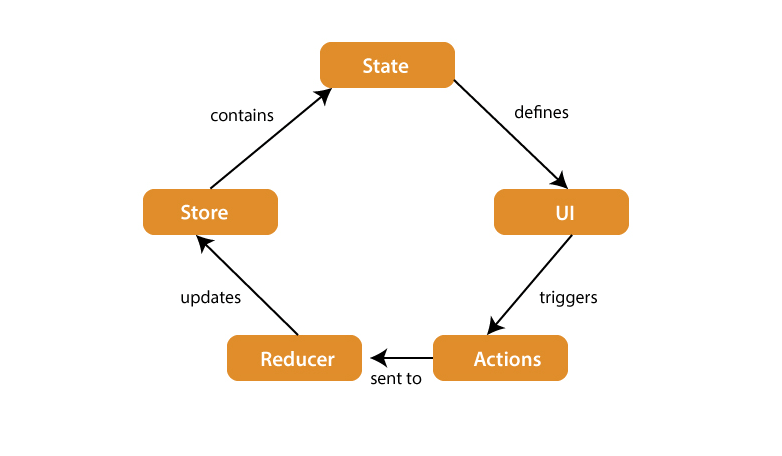
\includegraphics[width=1\linewidth]{redux-flow.png}
    \caption{Redux flow \cite{reduxFlow}}
    \label{fig:redux-flow}
\end{figure}

\subsubsection{Material UI}

\par Material UI (often abbreviated as MUI) is an open-source library that provides React components implementing Google's Material Design principles. Material Design is a design language developed by Google that emphasizes simplicity, consistency, and usability. Material-UI offers a comprehensive set of components and tools that help developers build aesthetically pleasing, responsive, and accessible user interfaces for web applications. Material UI provides various components like custom inputs, custom buttons, avatars, cards, dialogs, app bars, floating action buttons. Besides, it provides a powerful theming system that allows the customization of the appearance of components globally across the application, responsiveness through breakpoints and grids. It also includes a comprehensive set of Material Design icons that can be easily integrated into components. Icons are provided as React components and can be customized in terms of size, color, and other properties.

\begin{figure}[!ht]
    \centering
    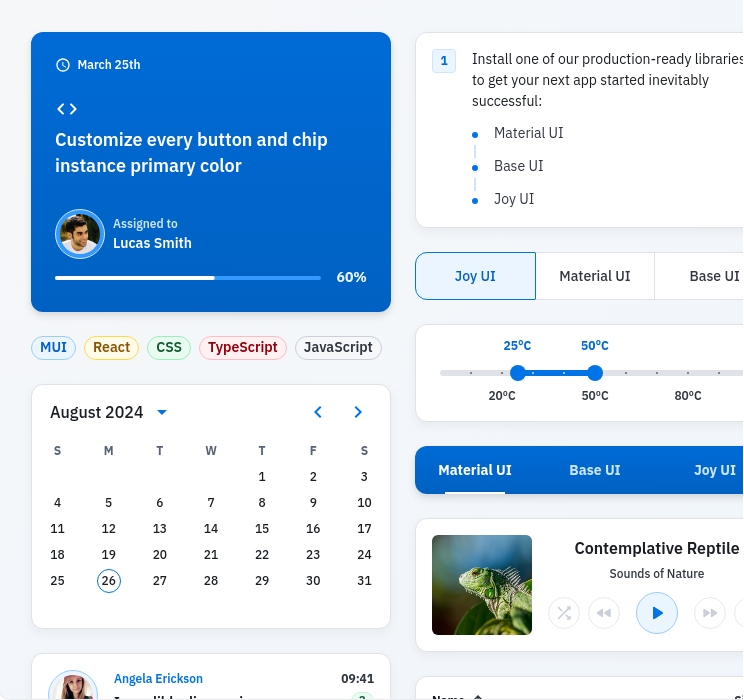
\includegraphics[width=1\linewidth]{material-ui-example.png}
    \caption{An example of what can be achieved with Material UI \cite{muiPreview}}
    \label{fig:enter-label}
\end{figure}